\documentclass{../../oss-apphys}

\begin{document}
\genheader

\gentitle{1 \& C}{SIMPLE HARMONIC MOTION \& UNIVERSAL GRAVITATION}{7 \& 8}

\genmultidirections

\gengravity

\raggedcolumns
\begin{multicols}{2}

  \begin{enumerate}[leftmargin=18pt]

  \item A simple pendulum has a mass $m$, length $L$, and period $T$. If the
    pendulum mass is replaced by a mass of $2m$, the period will be
    \begin{enumerate}[noitemsep,topsep=0pt,leftmargin=18pt,label=(\Alph*)]
    \item doubled
    \item halved
    \item quartered
    \item quadrupled
    \item unchanged
    \end{enumerate}

  \item A mass oscillates on the end of a spring that obeys Hooke's law. Which
    of the following statements is true?
    \begin{enumerate}[noitemsep,topsep=0pt,leftmargin=18pt,label=(\Alph*)]
    \item The amplitude of oscillation is equal to the potential energy of the
      spring.
    \item The kinetic energy of the oscillating mass is constant.
    \item Maximum potential energy occurs when the mass reaches the
      equilibrium position.
    \item The potential energy of the spring at the amplitude is equal to the
      kinetic energy at the equilibrium position.
    \item The kinetic energy of the spring at the amplitude is equal to the
      potential energy at the equilibrium position.
    \end{enumerate}

  \item A superball is dropped from a height of \SI{5.0}{\metre} above a floor.
    The ball bounces off the floor in a perfectly elastic collision so that it
    rises to the same height with each bounce. The motion of the ball can be
    described as
    \begin{enumerate}[noitemsep,topsep=0pt,leftmargin=18pt,label=(\Alph*)]
    \item harmonic motion with a period of $2$ \si{\second}
    \item harmonic motion with a period of $1$ \si{\second}
    \item harmonic motion with a period of $1/2$ \si{\second}
    \item motion with a constant velocity
    \item motion with a constant momentum
    \end{enumerate}

    \columnbreak
    
  \item An object oscillates in simple harmonic motion along the $x$-axis
    according to the equation $x=6 \cos(4t)$. The period of oscillation of the
    object is
    \begin{enumerate}[noitemsep,topsep=0pt,leftmargin=18pt,label=(\Alph*)]
    \item $1/4$ \si{\second}
    \item\SI{4}{\second}
    \item\SI{\pi/4}{\second}
    \item\SI{\pi/2}{\second}
    \item\SI{4\pi}{\second}
    \end{enumerate}    

  \item A mass $m$ oscillates on the end of a string of length $L$. The
    frequency of the pendulum is $f$. How would you increase the frequency of
    the pendulum to $2f$?
    \begin{enumerate}[noitemsep,topsep=0pt,leftmargin=18pt,label=(\Alph*)]
    \item Increase the length of the pendulum to $4L$
    \item Decrease the length of the pendulum to $1/4L$
    \item Increase the length of the pendulum to $2L$
    \item Decrease the length of the pendulum to $1/2L$
    \item Decrease the mass of the pendulum to $1/2m$
    \end{enumerate}

  \item A mass hangs from two parallel springs, each with the same spring
    constant $k$. Compared to the period $T$ of the same mass oscillating on
    one of the springs, the period of oscillation of the mass with both
    springs connected to it is
    \begin{center}
      \begin{tikzpicture}[scale=1.1]
        \fill [pattern=north east lines] (-2,4) rectangle (2,4.2);
        \draw[ultra thick] (-2,4)--(2,4);
        \draw[thick,
          decoration={aspect=0.3,segment length=2mm, amplitude=2.5mm, coil},
          decorate] (-1,4)--(-1,3);
        \draw[thick,
          decoration={aspect=0.3,segment length=2mm, amplitude=2.5mm, coil},
          decorate] (1,4)--(1,3);
        \draw[fill=gray!70](-1.5,3) rectangle(1.5,2);
      \end{tikzpicture}
    \end{center}
    \begin{enumerate}[noitemsep,topsep=0pt,leftmargin=18pt,label=(\Alph*)]
    \item $T/4$
    \item $T/2$
    \item $T$ (unchanged)
    \item $2T$
    \item $4T$
    \end{enumerate}

    \columnbreak
    
  \item Which of the following is generally true for an object in simple
    harmonic motion on a spring of constant $k$?
    \begin{enumerate}[noitemsep,topsep=0pt,leftmargin=18pt,label=(\Alph*)]
    \item The greater the spring constant $k$, the greater the amplitude of the
      motion.
    \item The greater the spring constant $k$, the greater the period of the
      motion.
    \item The greater the spring constant $k$, the greater the frequency of the
      motion.
    \item The lower the spring constant $k$, the greater the frequency of the
      motion.
    \item The lower the spring constant $k$, the greater the kinetic energy of
      the motion.
    \end{enumerate}
  \end{enumerate}

  \textbf{Questions 8 to 10}

  A harmonic oscillator follows the equation
  $\displaystyle\frac{d^2x}{dt^2}=-4x$. The spring constant $k$ is
  \SI{4}{\newton\per\metre}.
  
  \begin{enumerate}[leftmargin=18pt,resume]
  \item The angular frequency $\omega$ of the harmonic motion is
    \begin{enumerate}[noitemsep,topsep=0pt,leftmargin=18pt,label=(\Alph*)]
    \item zero
    \item\SI{2}{rad/s}
    \item\SI{4}{rad/s}
    \item\SI{8}{rad/s}
    \item\SI{16}{rad/s}
    \end{enumerate}

  \item The mass $m$ oscillating on the spring is
    \begin{enumerate}[noitemsep,topsep=0pt,leftmargin=18pt,label=(\Alph*)]
    \item\SI{1}{\kilo\gram}
    \item\SI{2}{\kilo\gram}
    \item\SI{4}{\kilo\gram}
    \item\SI{8}{\kilo\gram}
    \item\SI{16}{\kilo\gram}
    \end{enumerate}
  
  \item The period $T$ of oscillation is
    \begin{enumerate}[noitemsep,topsep=0pt,leftmargin=18pt,label=(\Alph*)]
    \item zero
    \item $\pi/4$\si{\second}
    \item $\pi/2$\si{\second}
    \item $\pi$  \si{\second}
    \item $2\pi$ \si{\second}
    \end{enumerate}

    \columnbreak
    
  \item A pendulum of length $L$ has a period of \SI{2}{\second} on Earth. A
    planetary explorer takes the same pendulum of length $L$ to another planet
    where its period is \SI{1}{\second}. The gravitational acceleration on the
    surface of this planet is most nearly
    \begin{enumerate}[noitemsep,topsep=0pt]
    \item $8 g$
    \item $4 g$
    \item $2 g$
    \item $1⁄2 g$
    \item $1⁄4 g$
    \end{enumerate}

  \item A block of mass \SI{1.}{\kilo\gram} is sliding on a frictionless
    horizontal surface with a speed of \SI{4.}{\metre\per\second} when it
    collides inelastically with another \SI{1.}{\kilo\gram} block attached to a
    spring. The spring compresses a distance of \SI{.5}{\metre} after the
    collision. The force constant $k$ of the spring is
    \begin{center}
      \begin{tikzpicture}
        \fill [pattern=north east lines](-5,0)--(0,0)--(0,2)--(0.2,2)
        --(0.2,-0.2)--(-5,-0.2)--cycle;
        \draw[ultra thick] (-5,0)--(0,0)--(0,2);
        \draw[decoration={aspect=0.3,segment length=2mm, amplitude=2.5mm, coil},
          decorate] (0,0.5)--(-1,0.5);
        \draw[fill=gray!70](-2,0) rectangle(-1,1)
        node[above]{\SI{1}{\kilo\gram}};
        \draw[fill=gray!70](-4.5,0) rectangle(-3.5,1)
        node[above]{\SI{1}{\kilo\gram}};
        \draw[ultra thick,->](-4,0.5)--(-2.8,0.5) node[pos=1,right]{$v$};
        \draw[very thick,dashed](-0.5,-0.5)--(-0.5,1.5);
      \end{tikzpicture}
    \end{center}
    \begin{enumerate}[noitemsep,topsep=0pt,leftmargin=18pt,label=(\Alph*)]
    \item\SI{2}{\newton\per\metre}
    \item\SI{4}{\newton\per\metre}
    \item\SI{8}{\newton\per\metre}
    \item\SI{16}{\newton\per\metre}
    \item\SI{32}{\newton\per\metre}
    \end{enumerate}

  \item A satellite orbits the Earth at a distance of \SI{100}{\kilo\metre}.
    The mass of the satellite is \SI{100}{\kilo\gram}, while the mass of the
    Earth is approximately \SI{6.e24}{\kilo\gram}. The radius of the Earth is
    approximately \SI{6.4e6}{\metre}. What is the approximate force of gravity
    acting on the satellite?
    \begin{enumerate}[noitemsep,topsep=0pt,leftmargin=18pt,label=(\Alph*)]
    \item\SI{4e4}{\newton}
    \item\SI{6.2e6}{\newton}
    \item\SI{4e8}{\newton}
    \item\SI{6.2e9}{\newton}
    \item\SI{4e14}{\newton}
    \end{enumerate}

    \columnbreak
    
  \item A block of mass \SI{.5}{\kilo\gram} rests up against a compressed
    spring of force constant \SI{5}{\newton\per\metre}. The spring is released,
    and the block travels a distance of \SI{1.}{\metre} when the block leaves
    the spring at the edge of the horizontal frictionless table, and is
    projected to the floor. The table is \SI{1.5}{\metre} high. The horizontal
    distance from the table the block lands on the floor is
    \begin{center}
      \pic{.4}{projectile.png}
    \end{center}
    \begin{enumerate}[noitemsep,topsep=0pt,leftmargin=18pt,label=(\Alph*)]
    \item\SI{1.2}{\metre}
    \item\SI{1.7}{\metre}
    \item\SI{2.1}{\metre}
    \item\SI{2.8}{\metre}
    \item\SI{3.4}{\metre}
    \end{enumerate}
%  \end{enumerate}
%
%\newpage
%\noindent The following questions are ``review'' questions for kinematics.
%
%\begin{enumerate}[leftmargin=50pt,label=\underline{\hspace{0.4in}} \arabic*.]
%  \setcounter{enumi}{13}
%
%\item  A golf ball is hit from level ground and has a horizontal range of
%  \SI{100}{\metre}. The ball leaves the golf club at an angle of \ang{60} to the
%  level ground. At what other angle(s) can the ball be struck at the same
%  initial velocity and still have a range of \SI{100}{\metre}?
%  \begin{enumerate}[noitemsep,topsep=0pt]
%  \item\ang{30}
%  \item\ang{20} and \ang{80}
%  \item\ang{10} and \ang{120}
%  \item\ang{45} and \ang{135}
%  \item There is no other angle other than \ang{60} in which the ball will have
%    a range of \SI{100}{\metre}.
%  \end{enumerate}
%
%  \vspace{-.23in}\begin{center}
%    \pic{0.3}{golf.png}
%  \end{center}
%
%\item\vspace{-.2in}A particle moves on a horizontal surface with a constant acceleration of
%  \SI{6}{m/s^2} in the $x$-direction and \SI{4}{m/s^2} in the $y$-direction. The
%  initial velocity of the particle is \SI{3}{\metre\per\second} in the $x$-direction.
%  The speed of the particle after \SI{4}{\second} is
%  \begin{enumerate}[noitemsep,topsep=0pt]
%  \item\SI{16}{\metre\per\second}
%  \item\SI{27}{\metre\per\second}
%  \item\SI{31}{\metre\per\second}
%  \item\SI{44}{\metre\per\second}
%  \item\SI{985}{\metre\per\second}
%  \end{enumerate}
%
%\item The displacement of the particle (from the previous question) from its
%  initial position is
%  \begin{enumerate}[noitemsep,topsep=0pt]
%  \item\SI{16}{\metre}
%  \item\SI{32}{\metre}
%  \item\SI{60}{\metre}
%  \item\SI{68}{\metre}
%  \item\SI{92}{\metre}
%  \end{enumerate}
%
%  \vspace{-0.5in}\begin{center}
%    \pic{0.3}{bounce.png}
%  \end{center}
%  
%\item\vspace{-.2in} A rubber ball is dropped from rest onto a plane angled at \ang{30} to the
%  horizontal floor and bounces off the plane with a horizontal speed $v_o$.
%  The ball lands on the plane a distance $D$ along the plane, as shown above.
%  In terms of $v_o$, $D$, and $g$, the speed of the ball just before striking
%  the plane is
%  \begin{enumerate}[noitemsep,topsep=0pt]
%  \item $v_o$
%  \item $\displaystyle\left(v_o^2+2D\sin\theta g\right)^\frac{1}{2}$
%  \item $\displaystyle\left(v_o+\frac{D\sin\theta}{g}\right)^\frac{1}{2}$
%  \item $\displaystyle\left(v_o^2+\frac{D\sin\theta}{g}\right)^\frac{1}{2}$
%  \item $\displaystyle\left(2D\sin\theta g\right)^\frac{1}{2}$
%  \end{enumerate}
%
%  \vspace{-.2in}\begin{center}
%    \pic{.55}{projectile2.png}
%  \end{center}
%
%\item\vspace{-.2in} A projectile is launched from a platform \SI{20}{\metre} high above level
%  ground. The projectile is launched with a velocity of \SI{40}{\metre\per\second} at an
%  angle of \ang{60} above the horizontal. The projectile follows a parabolic
%  path and reaches its original height at a horizontal distance of \SI{80}{\metre},
%  but moves past the height of the cliff to strike the ground below. The total
%  time from the launch until it strikes the ground is
%  \begin{enumerate}[noitemsep,topsep=0pt]
%  \item\SI{2}{\second}
%  \item\SI{4}{\second}
%  \item\SI{6}{\second}
%  \item\SI{9}{\second}
%  \item\SI{10}{\second}
%  \end{enumerate}
%
% \vspace{-.45in}\begin{center}
%   \pic{.45}{cup.png}
% \end{center}
%
%\item\vspace{-.2in}A small ball is launched with a speed of \SI{8}{\metre\per\second} at an angle of
%  \ang{30} from the horizontal. A cup is hung so that it is in position to
%  catch the ball when it reaches its maximum height. How far above the floor
%  should the cup be hung to catch the ball?
%  \begin{enumerate}[noitemsep,topsep=0pt]
%  \item\SI{2.4}{\metre}
%  \item\SI{1.6}{\metre}
%  \item\SI{1.0}{\metre}
%  \item\SI{0.8}{\metre}
%  \item\SI{0.4}{\metre}
%  \end{enumerate}
%
%\item A small airplane can fly at \SI{200}{km/h} with no wind. The pilot of the
%  plane would like to fly to a destination \SI{100}{\km} due north of his
%  present position, but there is a crosswind of \SI{50}{km/h} east. How much
%  time is required for the plane to fly north to its destination?
%  \begin{enumerate}[noitemsep,topsep=0pt]
%  \item less than \SI{1/2}{h}
%  \item \SI{1/2}{h}
%  \item more than \SI{1/2}{h}
%  \item \SI{1}{h}
%  \item more than \SI{1}{h}
%  \end{enumerate}
%
%  \item A car moves in a horizontal circle with a radius of \SI{10}{\metre}. The
%    tangential velocity of the car is \SI{30}{\metre\per\second}. What is the car's
%    acceleration?
%    \begin{enumerate}[noitemsep,topsep=0pt,leftmargin=18pt]
%    \item\SI{3}{m/s^2} toward the center
%    \item\SI{3}{m/s^2} away from the center
%    \item\SI{90}{m/s^2} toward the center
%    \item\SI{90}{m/s^2} away from the center
%    \item\SI{270}{m/s^2} toward the center
%    \end{enumerate}
  
  \item Two satellites of equal mass orbit a planet. Satellite B orbits at twice
    the orbital radius of Satellite A. Which of the following statements is
    true?
    \begin{enumerate}[noitemsep,topsep=0pt,leftmargin=18pt,label=(\Alph*)]
    \item The gravitational force on Satellite A is four times less than that on
      Satellite B.
    \item The gravitational force on Satellite A is two times less than that on
      Satellite B.
    \item The gravitational force on the satellites is equal.
    \item The gravitational force on Satellite A is two times greater than that
      on Satellite B.
    \item The gravitational force on Satellite A is four times greater than that
      on Satellite B.
    \end{enumerate}

    \columnbreak
    
  \item A $70$-\si{\kilo\gram} astronaut floats at a distance of \SI{10}{\metre}
    from a $50000$-\si{\kilo\gram} spacecraft. What is the force of attraction
    between the astronaut and spacecraft?
    \begin{enumerate}[noitemsep,topsep=0pt,leftmargin=18pt,label=(\Alph*)]
    \item\SI{2.4e-6}{\newton}
    \item\SI{2.4e-5}{\newton}
    \item Zero; there is no gravity in space.
    \item\SI{2.4e5}{\newton}
    \item\SI{2.4e6}{\newton}
    \end{enumerate}
    
  \item The centripetal acceleration on \SI{1000}{\kilo\gram} car in a turn is
    \SI{1e5}{m/s^2}. The radius of the turn is \SI{10}{\metre}. What is the
    car's speed?
    \begin{enumerate}[noitemsep,topsep=0pt,leftmargin=18pt,label=(\Alph*)]
    \item\SI{1e1}{\metre\per\second}
    \item\SI{1e2}{\metre\per\second}
    \item\SI{1e3}{\metre\per\second}
    \item\SI{1e4}{\metre\per\second}
    \item\SI{1e5}{\metre\per\second}
    \end{enumerate}
  
  \item A proposed ``space elevator'' can lift a \SI{1000}{\kilo\gram} payload
    to an orbit of \SI{150}{\kilo\metre} above the Earth's surface. The radius
    of the Earth is \SI{6.4e6}{\metre}, and the Earth's mass is
    \SI{6.e24}{\kilo\gram}. What is the gravitational potential energy of the
    payload when it reaches orbit?
    \begin{enumerate}[noitemsep,topsep=0pt,leftmargin=18pt,label=(\Alph*)]
    \item\SI{1.0e3}{\joule}
    \item\SI{2.7e6}{\joule}
    \item\SI{6.1e10}{\joule}
    \item\SI{2.7e12}{\joule}
    \item\SI{1.0e15}{\joule}
    \end{enumerate}

  \item The Earth is at an average distance of \SI{1}{AU} from the Sun and has
    an orbital period of \SI{1}{year}. Jupiter orbits the Sun at approximately
    \SI{5}{AU}. About how long is the orbital period of Jupiter?
    \begin{enumerate}[noitemsep,topsep=0pt,leftmargin=18pt,label=(\Alph*)]
    \item\SI{1}{year}
    \item\SI{2}{years}
    \item\SI{5}{years}
    \item\SI{11}{years}
    \item\SI{125}{years}
    \end{enumerate}

    \columnbreak
    
  \item A satellite orbits the Earth at a distance of \SI{200}{\km}. If the mass
    of the Earth is \SI{6.e24}{\kilo\gram} and the Earth's radius is
    \SI{6.4e6}{\metre}, what is the satellite's speed?
    \begin{enumerate}[noitemsep,topsep=0pt,leftmargin=18pt,label=(\Alph*)]
    \item\SI{1.e3}{\metre\per\second}
    \item\SI{3.5e3}{\metre\per\second}
    \item\SI{7.8e3}{\metre\per\second}
    \item\SI{5e6}{\metre\per\second}
    \item\SI{6.1e7}{\metre\per\second}
    \end{enumerate}
  
  \item Mars orbits the Sun at a distance of \SI{2.3e11}{\metre}. The mass of
    the Sun is \SI{2.e30}{\kilo\gram}, and the mass of Mars is
    \SI{6.4e23}{\kilo\gram}. Approximately what is the gravitational force that
    the Sun exerts on Mars?
    \begin{enumerate}[noitemsep,topsep=0pt,leftmargin=18pt,label=(\Alph*)]
    \item\SI{1.6e20}{\newton}
    \item\SI{1.6e21}{\newton}
    \item\SI{3.7e21}{\newton}
    \item\SI{3.7e32}{\newton}
    \item\SI{3.7e42}{\newton}
    \end{enumerate}

  \item When climbing from sea level to the top of Mount Everest, a hiker
    changes elevation by \SI{8848}{\metre}. By what percentage will the
    gravitational field of the Earth change during the climb? (The Earth's
    mass is \SI{6.e24}{\kilo\gram}, and its radius is \SI{6.4e6}{\metre}.)
    \begin{enumerate}[noitemsep,topsep=0pt,leftmargin=18pt,label=(\Alph*)]
    \item It will increase by approximately \SI{0.3}{\percent}.
    \item It will decrease by approximately \SI{0.3}{\percent}.
    \item It will increase by approximately \SI{12}{\percent}.
    \item It will decrease by approximately \SI{12}{\percent}.
    \item The gravitational field strength will not change.
    \end{enumerate}

  \item Four planets, A through D, orbit the same star. The relative masses and
    distances from the star for each planet are shown in the table. For
    example, Planet A has twice the mass of Planet B, and Planet D has
    three times the orbital radius of Planet A. Which planet has the highest
    gravitational attraction to the star?
    \begin{center}
      \vspace{-.1in}
      \begin{tabular}{lll}
        \hline
        \textbf{Planet} & \textbf{Relative mass} & \textbf{Relative distance}\\
        \hline
        A\hspace{.4in}& $2m$     & $r$    \\ \hline
        B & $m$                  & $0.1r$\hspace{.25in} \\ \hline
        C & $0.5m$\hspace{.25in} & $2r$   \\ \hline
        D & $4m$                 & $3r$   \\ \hline
      \end{tabular}
    \end{center}
    \begin{enumerate}[noitemsep,topsep=0pt,leftmargin=18pt,label=(\Alph*)]
    \item Planet A
    \item Planet B
    \item Planet C
    \item Planet D
    \item All have the same gravitational attraction to the star.
    \end{enumerate}

  \item A satellite orbits the Earth at a distance that is four times the radius
    of the Earth. If the acceleration due to gravity near the surface of the
    Earth is $g$, the acceleration of the satellite is most nearly
    \begin{enumerate}[noitemsep,topsep=0pt,leftmargin=18pt,label=(\Alph*)]
    \item zero
    \item $g/2$
    \item $g/4$
    \item $g/8$
    \item $g/16$
    \end{enumerate}

  \item The mass of a planet is $1/4$ that of Earth and its radius is half of
    Earth's radius. The acceleration due to gravity on this planet is most
    nearly
    \begin{enumerate}[noitemsep,topsep=0pt,leftmargin=18pt,label=(\Alph*)]
    \item\SI{2 }{\metre\per\second^2}
    \item\SI{4 }{\metre\per\second^2}
    \item\SI{5 }{\metre\per\second^2}
    \item\SI{10}{\metre\per\second^2}
    \item\SI{20}{\metre\per\second^2}
    \end{enumerate}
  
  \item A satellite orbits the Earth in an elliptical orbit, with point A being
    close to the Earth and point B farther away. As the satellite moves from
    point A to point B, which of the following is true of the angular momentum
    and kinetic energy of the satellite?
    \begin{center}
      \vspace{-.1in}
      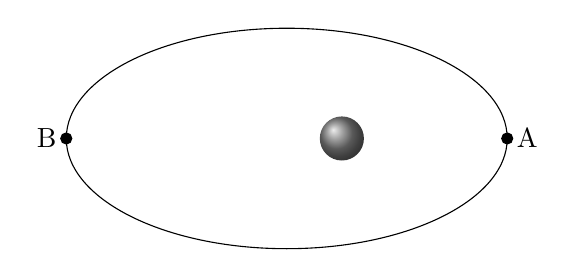
\begin{tikzpicture}[scale=1.4]
        \tikzstyle{balloon}=[ball color=gray];
        \draw(0,0) ellipse (2 and 1);
        \draw[fill=black](2,0) circle(0.05) node[right]{A};
        \draw[fill=black](-2,0) circle(0.05) node[left]{B};
        \shade[balloon] (0.5,0) circle (0.2);
      \end{tikzpicture}
    \end{center}
  
    \begin{tabular}{lll}
      & \underline{Angular momentum} & \underline{Kinetic energy}\\
      (a) & Increases & Remains constant \\
      (b) & Remains constant & Increases \\
      (c) & Decreases & Remains constant \\
      (d) & Remains constant & Decreases \\
      (e) & Remains constant & Remains constant
    \end{tabular}

  \item Two planets of mass $M$ and $9M$ are in the same solar system. The
    radius of the planet of mass $M$ is $R$. In order for the acceleration due
    to gravity to be the same for each planet, the radius of the planet of mass
    $9M$ would have to be
    \begin{enumerate}[noitemsep,topsep=0pt,leftmargin=18pt,label=(\Alph*)]
    \item $R/2$
    \item $R$
    \item $2R$
    \item $3R$
    \item $9R$
    \end{enumerate}
    \vspace{-.5in}
  \item Two planets, X and Y, orbit a star. Planet X orbits at a radius $R$, and
    Planet Y orbits at a radius $3R$. Which of the following best represents
    the relationship between the acceleration $a_X$ of Planet X and the
    acceleration $a_Y$ of Planet Y?
    \begin{center}
      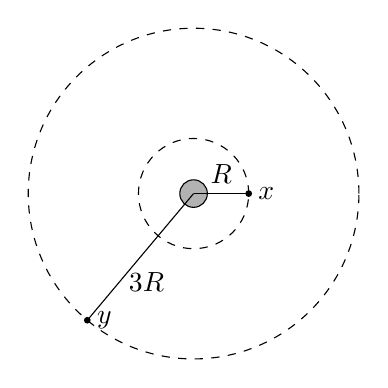
\begin{tikzpicture}[scale=.7]
        \draw[fill=gray!60](0,0) circle(0.25);
        \draw[dashed](0,0) circle(1);
        \draw[dashed](0,0) circle(3);
        \draw(0,0)--(1,0) node[pos=1,right]{$x$} node[midway,above]{$R$};
        \draw[fill=black](1,0) circle(0.05);
        \begin{scope}[rotate=230]
          \draw(0,0)--(3,0) node[pos=1,right]{$y$} node[pos=0.7,right]{$3R$};
          \draw[fill=black](3,0) circle(0.05);
        \end{scope}
      \end{tikzpicture}
    \end{center}
    \begin{enumerate}[noitemsep,topsep=0pt,leftmargin=18pt,label=(\Alph*)]
    \item $a_X = 9a_Y$
    \item $9a_X = a_Y$
    \item $a_X = 3a_Y$
    \item $3a_X = a_Y$
    \item $a_X = a_Y$
    \end{enumerate}
  \item A satellite is in a stable circular orbit around the Earth at a radius
    $R$ and speed $v$. At what radius would the satellite travel in a stable
    orbit with a speed $2v$?
    \begin{enumerate}[noitemsep,topsep=0pt,leftmargin=18pt,label=(\Alph*)]
    \item $1⁄4\;R$
    \item $1⁄2\;R$
    \item $R$
    \item $2R$
    \item $4R$
    \end{enumerate}

  \item The Earth and the moon apply a gravitational force to each other.
    Which of the following statements is true?
    \begin{enumerate}[noitemsep,topsep=0pt,leftmargin=18pt,label=(\Alph*)]
    \item The Earth applies a greater force on the moon than the moon exerts on
      the Earth.
    \item The Earth applies a smaller force on the moon than the moon exerts on
      the Earth.
    \item The Earth applies a force on the moon, but the moon does not exert a
      force on the Earth.
    \item The Earth does not apply a force on the moon, but the moon exerts a
      force on the Earth.
    \item The force the Earth applies to the moon is equal and opposite to the
      force the moon applies to the Earth.
    \end{enumerate}

    \columnbreak
    
  \item Two masses exert a gravitational force $F$ on each other. If one of the
    masses is doubled, and the distance between the masses is tripled, the
    new force between them is
    \begin{enumerate}[noitemsep,topsep=0pt,leftmargin=18pt,label=(\Alph*)]
    \item $6F$
    \item $2F/3$
    \item $2F/9$
    \item $3F/2$
    \item $4F/9$
    \end{enumerate}

  \item A planet orbits at a radius $R$ around a star of mass $M$. The period of
    orbit of the planet is
    \begin{enumerate}[noitemsep,topsep=0pt,leftmargin=18pt,label=(\Alph*)]
    \item $\displaystyle\sqrt{\frac{4\pi^2R^2}{GM}}$
    \item $\displaystyle\frac{4\pi^2R^3}{GM}$
    \item $\displaystyle\sqrt{\frac{4\pi^2R^3}{GM}}$
    \item $\displaystyle\sqrt{\frac{4\pi^2R}{GM}}$
    \item $\displaystyle\frac{GM}{4\pi^2R}$
    \end{enumerate}
  
  \item A moon orbits a large planet in an elliptical orbit, with its closest
    approach at a distance $a$, and its farthest distance $b$. The speed of the
    moon at point b is $v$. The speed at point $a$ is
    \begin{enumerate}[noitemsep,topsep=0pt,leftmargin=18pt,label=(\Alph*)]
    \item $\displaystyle\frac{av}{b}$
    \item $\displaystyle\frac{bv}{a}$
    \item $\displaystyle\frac{(a+b)v}{b}$
    \item $\displaystyle\frac{(b-a)v}{b}$
    \item $\displaystyle\frac{2bv}{a}$
    \end{enumerate}

    \columnbreak
    
  \item A satellite orbits the Earth in an elliptical orbit. Which of the
    following statements is true?
    \begin{enumerate}[noitemsep,topsep=0pt,leftmargin=18pt,label=(\Alph*)]
    \item The angular velocity of the satellite increases as it travels farther
      from the Earth.
    \item The acceleration of the satellite increases as it travels closer to
      the Earth.
    \item The angular momentum of the satellite increases as it travels closer
      to the Earth.
    \item The potential energy of the satellite is equal to its kinetic energy
      at all points in the orbit.
    \item The speed of the satellite must remain constant for it to remain
      in orbit around the Earth.
    \end{enumerate}

  \item Two moons of mass $m$ and $2m$ orbit a planet of mass $M$
    at the same radius $R$ and speed $v$ toward each other, as shown. The moons
    collide and stick together without destroying either moon. The total
    momentum of the moons after the collision is
    \begin{center}
      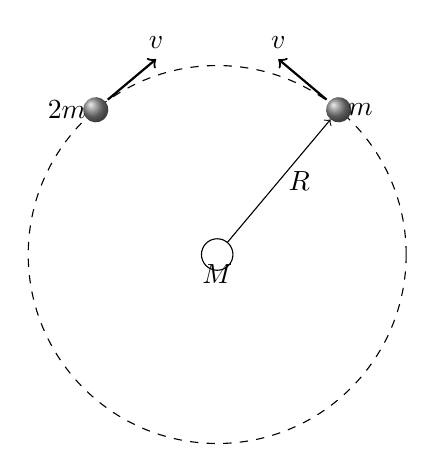
\begin{tikzpicture}[scale=0.8]
        \tikzstyle{balloon}=[ball color=gray];
        \draw(0,0) circle(0.25);
        \draw[dashed](0,0) circle(3) node[below]{$M$};
        \begin{scope}[rotate=50]
          \draw[->](0.25,0)--(2.8,0) node[midway,right]{$R$};
          \shade[balloon] (3,0) circle (0.2) node[right]{$m$};
          \draw[thick,->](3,0.25)--(3,1.25) node[pos=1,above]{$v$};
        \end{scope}
        \begin{scope}[rotate=130]
          \shade[balloon] (3,0) circle (0.2) node[left]{$2m$};
          \draw[thick,->](3,-0.25)--(3,-1.25) node[pos=1,above]{$v$};
        \end{scope}
      \end{tikzpicture}
    \end{center}
    \begin{enumerate}[noitemsep,topsep=0pt,leftmargin=18pt,label=(\Alph*)]
    \item $mv$
    \item $2mv$
    \item $3mv$
    \item $6mv$
    \item zero
    \end{enumerate}

    \columnbreak
    
  \item The velocity of the two masses after the collision above is
    \begin{enumerate}[noitemsep,topsep=0pt,leftmargin=18pt,label=(\Alph*)]
    \item $v$ counterclockwise
    \item $v/2$ counterclockwise
    \item $v/2$ clockwise
    \item $v/3$ counterclockwise
    \item $v/3$ clockwise
    \end{enumerate}

  \item Consider a two-star system shown above, which consists of two stars of
    mass $m$ rotating in a circle of radius $r$ about their center of mass. What
    is the total energy of the two-star system?
    \begin{enumerate}[noitemsep,topsep=0pt,leftmargin=18pt,label=(\Alph*)]
    \item $-Gm^2/2r$
    \item $Gm^2/2r$
    \item $Gm^2/4r$
    \item $3Gm^2/4r$
    \item $-Gm^2/4r$
    \end{enumerate}

  \item If a planet has twice the radius of Earth and half of Earth's density,
    what is the acceleration due to gravity on the surface of the planet (in
    terms of the gravitational acceleration $g$ on the surface of Earth)?
    \begin{enumerate}[noitemsep,topsep=0pt,leftmargin=18pt,label=(\Alph*)]
    \item $4g$
    \item $2g$
    \item $g$
    \item $g/2$
    \item $g/4$
    \end{enumerate}
  \end{enumerate}
\end{multicols}

\newpage
\genanswersheet{1 \& C}{Simple Harmonic Motion and Universal Gravitation}

\begin{center}
  \begin{minipage}[t]{.2\textwidth}
    \vspace{.2in}
    \bgroup
    \begin{tabular}{>{\centering}m{1.3cm} >{\centering}m{1.7cm}}
      No. & Answer
    \end{tabular}\\
    \def\arraystretch{1.5}
    \begin{tabular}{|>{\centering}m{1.3cm}|>{\centering}m{1.7cm}|}
      \hline
      1 & \\ \hline
      2 & \\ \hline
      3 & \\ \hline
      4 & \\ \hline
      5 & \\ \hline
      6 & \\ \hline
      7 & \\ \hline
      8 & \\ \hline
      9 & \\ \hline
      10 & \\ \hline
      11 & \\ \hline
      12 & \\ \hline
      13 & \\ \hline
      14 & \\ \hline
      15 & \\ \hline
      16 & \\ \hline
      17 & \\ \hline
      18 & \\ \hline
      19 & \\ \hline
      20 & \\ \hline
      21 & \\ \hline
      22 & \\ \hline
      23 & \\ \hline
      24 & \\ \hline
      25 & \\ \hline
    \end{tabular}
    \egroup
  \end{minipage}
  \hspace{.5in}
  \begin{minipage}[t]{.2\textwidth}
    \vspace{.2in}
    \bgroup
    \begin{tabular}{>{\centering}m{1.3cm} >{\centering}m{1.7cm}}
      No. & Answer
    \end{tabular}\\
    \def\arraystretch{1.5}
    \begin{tabular}{|>{\centering}m{1.3cm}|>{\centering}m{1.7cm}|}
      \hline
      26 & \\ \hline
      27 & \\ \hline
      28 & \\ \hline
      29 & \\ \hline
      30 & \\ \hline
      31 & \\ \hline
      32 & \\ \hline
      33 & \\ \hline
      34 & \\ \hline
      35 & \\ \hline
      36 & \\ \hline
      37 & \\ \hline
      38 & \\ \hline
    \end{tabular}
    \egroup
  \end{minipage}
\end{center}
\newpage

\genfreetitle{1 \& C}{SIMPLE HARMONIC MOTION \& UNIVERSAL GRAVITATION}{5}

\genfreedirections{10}

\begin{enumerate}[leftmargin=15pt]

\item A mass $m$ oscillates on an ideal spring of spring constant $k$ on a
  frictionless horizontal surface. The mass is pulled aside to a distance $A$
  from its equilibrium position, and released.
  \begin{center}
    \begin{tikzpicture}[scale=.9]
      \fill [pattern=north east lines] (5,0)--(0,0)--(0,2)--(-0.2,2)
      --(-0.2,-0.2)--(5,-0.2)--cycle;
      \draw[ultra thick] (5,0)--(0,0)--(0,2)--(-0.5,2);
      \draw[decoration={aspect=0.3,segment length=2mm, amplitude=2.5mm, coil},
        decorate] (0,0.5)--(1.5,0.5);
      \draw[fill=gray!70](1.5,0) rectangle(2.5,1);
      \draw[thick](2.5,0)--(2.5,-0.3) node[pos=1,below]{O};
      \draw[thick](4,0)--(4,-0.3) node[pos=1,below]{A};
    \end{tikzpicture}
  \end{center} 
  \begin{enumerate}[noitemsep]  
  \item\vspace{-.15in} In terms of the given quantities, at what distance from
    the equilibrium
    position is the potential energy of the mass equal to its kinetic energy?
  \item In terms of the given quantities, what is the acceleration of the mass
    when it is at the amplitude $A$?
  \end{enumerate}
  \vspace{1.6in}
  %\newpage
  
\item A mass oscillates in simple harmonic motion as shown by the position $x$
  vs. time $t$ graph below.
  \begin{center}
    \vspace{-.1in}\pic{.3}{oscillate.png}
  \end{center}
  \begin{enumerate}[noitemsep]  
  \item What is the frequency of oscillation?
  \item Write the equation that represents the speed of the mass as a function
    of time.
  \end{enumerate}
  \newpage

%\item The acceleration vs.\ time graph shows the motion of an elevator during a
%  $20$-second time interval. The elevator starts from rest at time $t=0$. 
%  \begin{center}
%    \pic{.7}{a-t.png}
%  \end{center}
%  \begin{enumerate}[noitemsep]
%  \item Determine the instantaneous velocity of the elevator at the end of
%    \SI{10}{\second}.
%    \vspace{1.5in}
%  \item Determine the displacement of the elevator after \SI{5}{\second}.
%    \vspace{1.5in}
%  \item On the axes below, sketch the graph that represents the velocity vs.\
%    time graph for the elevator for the $20$-second time interval.
%    \begin{center}
%      \pic{.7}{v-t.png}
%    \end{center}
%    \newpage
%  \end{enumerate}
  
%\item A particle follows a parabolic path with the equation $y=2x^2$ as shown.
%  The $x$-component of the particle's velocity $v_x$ as a function of time $t$
%  is $6$, that is, the horizontal displacement is $x=6t$.
%  \begin{center}
%    \begin{tikzpicture}
%      \draw[very thick,->](0,0)--(5,0) node[pos=1,right]{$x$};
%      \draw[very thick,->](0,0)--(0,4) node[pos=1,above]{$y$};
%      \draw[very thick,smooth,samples=20,domain=0:4.2] plot(\x,{.2*\x*\x});
%      \draw[fill=black](3,1.8) circle(0.05) node[right]{$P$};
%    \end{tikzpicture}
%  \end{center}
%  \begin{enumerate}[noitemsep]
%  \item Determine the $y$-component of the particle's velocity $v_y$ as a
%    function of time.
%  \item On the diagram above, sketch arrows to represent the horizontal and
%    vertical components of the particle's acceleration at point $P$.
%  \end{enumerate}
%  \vspace{1in}
  
\item A spacecraft moving with an initial velocity $\mb{v}_0$, shown below,
  ``slingshots'' around the sun in order to reverse its direction. The sun's
  mass is $m_\mathrm{sun}$ and you can make the assumption that the sun remains
  stationary.\\
  \begin{minipage}{0.28\textwidth}
    \pic{1}{shuttle.jpg}
  \end{minipage}
  \begin{minipage}{0.7\textwidth}
    \begin{enumerate}[noitemsep]
    \item What is the minimum initial speed required by the spacecraft to escape
      the sun's gravitational field and move in a trajectory toward infinity?
    \item What is the minimum initial speed $v_o$ that the spacecraft must have
      in order to avoid falling into the sun? (Treat the sun and the spacecraft
      as points.)
    \item Repeat the previous questions, but now the sun has a radius $R$.
    \item Write down the equations required to calculate the initial angle
      $\theta$ in terms of $v_0$, $d$, $m_\mathrm{sun}$, $G$, and $r$.
    \end{enumerate}
  \end{minipage}
  \newpage
\item A planet of mass $M$, radius $R$, and uniform density has a small tunnel
  drilled through the center of the planet, as shown below. When the mass is
  inside the tunnel, it experiences a force of $F=(GmM/R^3)r$, whereas when the
  mass is outside of the planet, it experiences a gravitational force of
  $F=GmM/r^2$.
  \begin{center}
    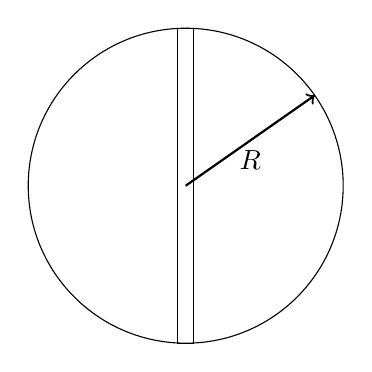
\begin{tikzpicture}
      \draw(0,0) circle(2);
      \draw(-0.1,2) rectangle(0.1,-2);
      \draw[->,thick,rotate=35](0,0)--(2,0) node[midway,below]{$R$};
    \end{tikzpicture}
  \end{center}
  \begin{enumerate}[noitemsep,leftmargin=20pt]
  \item Setting the potential energy of the mass to be zero at the planet's
    center, calculate the mass's potential energy as a function of distance from
    the center of the planet $U(r)$, for values $r<R$. Sketch this potential
    function.
  \item If the mass is dropped from $R$ from the center of the planet, how long
    will it take until it returns to its original position?
  \item If the mass is dropped from $R/2$ from the center of the planet, will
    it require more, or less, or the same amount of time to return to its
    original position compared to if it was dropped from $R$?
  \item If the mass is dropped from $2R$ from the center of the planet, will
    it require more, or less, or the same amount of time to return to its
    original position compared to if it was dropped from $R$?
  \end{enumerate}
  \newpage
\item Two stars of unequal mass orbit each other about their common center of
  mass as shown. The star of mass $M_1$ orbits in a circle of radius $r$, and
  the star of mass $M_2$ orbits in a circle of radius $2r$.
  \begin{center}
    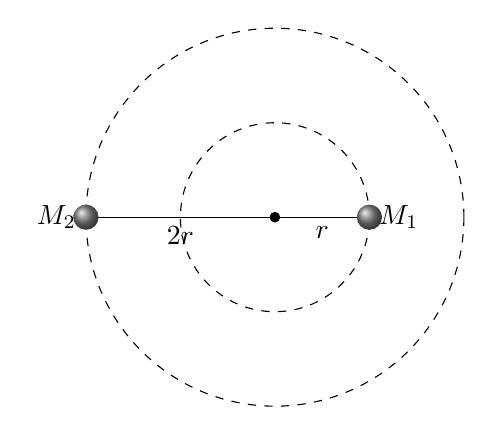
\begin{tikzpicture}[scale=0.8]
      \tikzstyle{balloon}=[ball color=gray];
      \draw[fill=black](0,0) circle(0.075);
      \draw[dashed](0,0) circle(3);
      \draw[dashed](0,0) circle(1.5);
      \draw[->](0,0)--(1.5,0) node[midway,below]{$r$};
      \shade[balloon] (1.5,0) circle (0.2) node[right]{$M_1$};
      \draw[->](0,0)--(-3,0) node[midway,below]{$2r$};
      \shade[balloon] (-3,0) circle (0.2) node[left]{$M_2$};
    \end{tikzpicture}
  \end{center}
  \begin{enumerate}[noitemsep,leftmargin=20pt]
  \item Determine the ratio of masses $M_1/M_2$.
  \item Determine the ratio of the acceleration $a_1$ of $M_1$ to the
    acceleration $a_2$ of $M_2$.
  \item Determine the ratio of the period $T_1$ of $M _1$ to the period $T_2$
    of $M_2$.
  \end{enumerate}

\end{enumerate}
\end{document}
